\documentclass[a4paper,12pt]{article}
\usepackage{../../mypackages}
\usepackage{../../macros}


\begin{document}

\title{Chapitre 4 : L'atome}
\author{N. Bancel}
\date{Octobre 2024}
\maketitle

\section{Exercices}

\subsection{Alcool}


\begin{figure}[H]
  \centering
  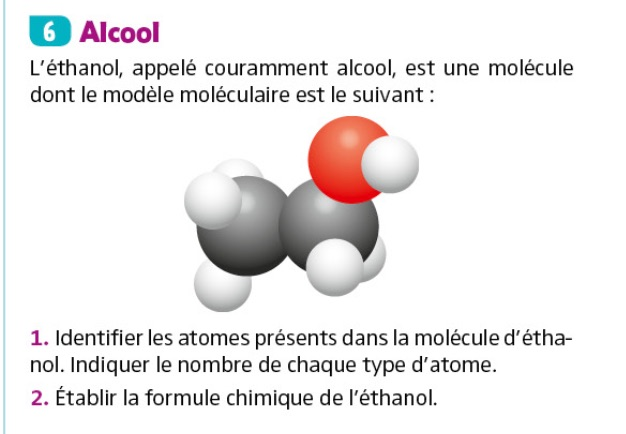
\includegraphics[width=0.7\linewidth]{04_01_01.jpg}
\end{figure}



\begin{enumerate}
  \item \textbf{Identification des atomes et leur nombre dans la molécule d'éthanol}
  
  La molécule d'éthanol est composée des éléments suivants :
  \begin{itemize}[noitemsep]
      \item Atomes de carbone (C)
      \item Atomes d'hydrogène (H)
      \item Atomes d'oxygène (O)
  \end{itemize}
  
  En analysant le modèle moléculaire, on peut compter :
  \begin{itemize}[noitemsep]
      \item 2 atomes de carbone (C)
      \item 6 atomes d'hydrogène (H)
      \item 1 atome d'oxygène (O)
  \end{itemize}
  
  \item \textbf{Formule chimique de l'éthanol}
  
  La formule chimique d'une molécule se base sur la quantité de chaque type d'atome présent. Pour l'éthanol, qui est composé de 2 atomes de carbone, 6 atomes d'hydrogène et 1 atome d'oxygène, la formule est donnée par :
  \[
  C_2H_6O
  \]
  
 Les lettres sont ordonnées dans l'ordre alphabétique
\end{enumerate}

\subsection{Test de connaissances}


\begin{figure}[H]
  \centering
  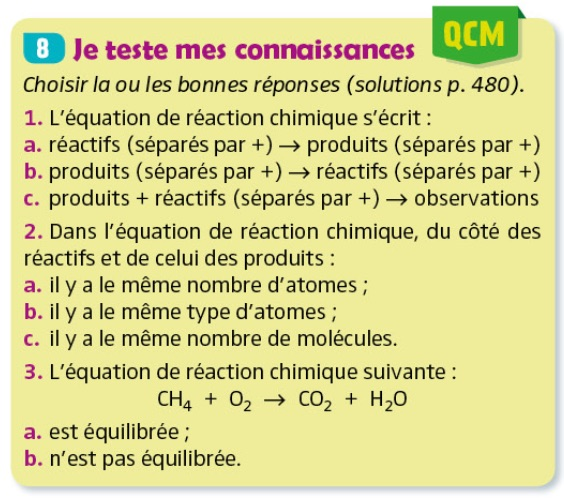
\includegraphics[width=0.7\linewidth]{04_01_02.jpg}
\end{figure}


\begin{enumerate}
  \item \textbf{L'equation de reaction chimique s'ecrit :} \\
  \textbf{Réponse :} a. Réactifs (separes par +) $\rightarrow$ produits (separes par +). \\
  \textit{Justification :} Une équation chimique décrit le processus de transformation des réactifs en produits. Les réactifs sont toujours placés à gauche de la flèche et les produits à droite.

  \item \textbf{Dans l'\'equation de r\'eaction chimique, du c\^ot\'e des r\'eactifs et de celui des produits :} \newline
  \textbf{Réponse :} a. il y a le m\^eme nombre d'atomes. \newline
  \textit{Justification :} La loi de conservation de la masse stipule que le nombre d'atomes de chaque élément doit être le même des deux côtés de l'équation chimique. Cela garantit que la matière n'est ni créée ni détruite.

  \item \textbf{L'equation de reaction chimique suivante : $\ce{CH4 + O2 -> CO2 + H2O}$} \newline
  \textbf{Réponse :} b. n'est pas equilibree. \newline
  \textit{Justification :} Comptons le nombre d'atomes de chaque côté :
  \begin{itemize}
      \item \textbf{Côté réactifs :} 1 atome de carbone (C), 4 atomes d'hydrogène (H) et 2 atomes d'oxygène (O) par molécule de O$_2$ (donc 2 $\times$ 1 = 2).
      \item \textbf{Côté produits :} 1 atome de carbone (C) dans CO$_2$, 2 atomes d'oxygène (O) dans CO$_2$ et 2 atomes d'hydrogène (H) et 1 atome d'oxygène (O) dans H$_2$O.
  \end{itemize}
  \textbf{Analyse :} On constate que le côté des réactifs contient 2 atomes d'oxygène, alors que le côté des produits en contient 3 (2 dans CO$_2$ + 1 dans H$_2$O). L'hydrogène est équilibré, mais l'oxygène ne l'est pas, prouvant ainsi que l'équation n'est pas équilibrée
\end{enumerate}

\subsection{La rouille}

La formation de la rouill provient d'une réaction chimique entre le fer et le dioxygène de l'air.

\begin{enumerate}

 \item Ecrire l'équation de réaction chimique en toutes lettres
 
 La rouille se forme lorsqu'il y a une réaction entre le fer (Fe) et le dioxygène ($O_2$) présent dans l'air. Cette réaction chimique donne de la rouille. L'équation en toutes lettres est :
 \[
 \text{Fer + Dioxygène} \rightarrow \text{Rouille}
 \]

 \item Parmi les équations de réaction de formation de la rouille ci-dessous, identifier celle qui est équilibrée 
 
 \begin{itemize}[noitemsep]
  \item[A] \ce{Fe + O2 -> Fe2O3}
  \item[B] \ce{2 Fe + 3 O2 -> Fe2O3}
  \item[C] \ce{4 Fe + 3 O2 -> 2 Fe2O3}
 \end{itemize}

 Pour qu'une équation chimique soit équilibrée, le nombre d'atomes de chaque élément doit être identique de part et d'autre de la réaction. Analysons les équations données :
    
 \begin{itemize}
     \item[A] \ce{Fe + O2 -> Fe2O3} \\
     Cette équation n'est pas équilibrée : il y a 2 atomes de fer à droite mais seulement 1 à gauche, et 3 atomes d'oxygène à droite mais 2 à gauche.
     
     \item[B] \ce{2 Fe + 3 O2 -> Fe2O3} \\
     Cette équation n'est pas équilibrée : il y a 2 atomes de fer à gauche mais 2 à droite, mais 3 molécules de dioxygène à gauche, soit 6 atomes, ce qui ne correspond pas aux 3 atomes à droite.
     
     \item[C] \ce{4 Fe + 3 O2 -> 2 Fe2O3} \\
     Cette équation est équilibrée : il y a 4 atomes de fer de chaque côté et 6 atomes d'oxygène de chaque côté.
 \end{itemize}

 \textcolor{orange}{\textbf{Conclusion / Interprétation}} \\
 L'équation de réaction correctement équilibrée est l'option \textbf{C} : \\
\ce{4 Fe + 3 O2 -> 2 Fe2O3}.
 

\end{enumerate}



\subsection{Photosynthèse}

Un élève de biologie a écrit l'équation de la photosynthèse (la transformation chimique à la base de la croissance des plantes), de la façon suivante : \par 
\[
\ce{6CO2 + 6H2O -> C6H12O6 + 6O2}
\]
 
\begin{itemize}[noitemsep]
  \item[1] Identifier les réactions et les produits. Les nommer. \ce{C6H12O6} est la molécule du sucre
  \item[2] Cette équation est-elle équilibrée ? 
 \end{itemize}

\textcolor{orange}{\textbf{Correction}}

\begin{itemize}

  \item[1] \textbf{Identification des réactifs et des produits} \\
    Les réactifs sont les substances initiales présentes avant la réaction chimique, tandis que les produits sont les substances formées après la réaction.
    \begin{itemize}
        \item \textbf{Réactifs} : 
        \begin{itemize}
            \item \ce{CO2} : Dioxyde de carbone
            \item \ce{H2O} : Eau
        \end{itemize}
        
        \item \textbf{Produits} :
        \begin{itemize}
            \item \ce{C6H12O6} : Glucose (sucre)
            \item \ce{O2} : Dioxygène
        \end{itemize}
    \end{itemize}

    \item[2] \textbf{Vérification de l'équilibre de l'équation}
    
    Une équation chimique est équilibrée lorsque le nombre d'atomes de chaque élément est le même des deux côtés de l'équation. Analysons l'équation donnée :
    \[
    \ce{6CO2 + 6H2O -> C6H12O6 + 6O2}
    \]

    Comptons les atomes de chaque côté :
    \begin{itemize}[noitemsep]
        \item \textbf{Côté gauche (réactifs)} :
        \begin{itemize}
            \item Carbone (C) : $6 \times 1 = 6$
            \item Hydrogène (H) : $6 \times 2 = 12$
            \item Oxygène (O) : $6 \times 2 + 6 \times 1 = 18$
        \end{itemize}
        
        \item \textbf{Côté droit (produits)} :
        \begin{itemize}
            \item Carbone (C) : $1 \times 6 = 6$
            \item Hydrogène (H) : $1 \times 12 = 12$
            \item Oxygène (O) : $6 \times 1 + 6 \times 2 = 18$
        \end{itemize}
    \end{itemize}
    
    \textcolor{blue}{\textbf{Conclusion / Interprétation}} \\
    L'équation est bien équilibrée : le nombre d'atomes de carbone, d'hydrogène et d'oxygène est le même des deux côtés de l'équation.
    
\end{itemize}

\end{document}
